\documentclass[openany]{book}

\input{../../../latex_preambule_style/preambule}
\input{../../../latex_preambule_style/styleCoursCycle4}
\input{../../../latex_preambule_style/styleExercices}
\input{../../../latex_preambule_style/styleExercicesAideCompetences}
%\input{../../latex_preambule_style/styleCahier}
\input{../../../latex_preambule_style/bas_de_page_cycle4}
\input{../../../latex_preambule_style/algobox}


%%%%%%%%%%%%%%%  Affichage ou impression  %%%%%%%%%%%%%%%%%%
\newcommand{\impress}[2]{
\ifthenelse{\equal{#1}{1}}  %   1 imprime / affiche sur livre  -----    0 affiche sur cahier 
{%condition vraieé
#2
}% fin condition vraie
{%condition fausse
}% fin condition fausse
} % fin de la procédure
%%%%%%%%%%%%%%%  Affichage ou impression  %%%%%%%%%%%%%%%%%%
 \usepackage{geometry}
 \geometry{top=2cm, bottom=0cm, left=2cm , right=2cm}
%%%%%%%%%%%%%%%%%%%%%%%%%%%%%%%%%%%%%%%%%%%%%%%%

\begin{document}





\paragraphe{Repère dans l'espace}

\begin{DefT}{coordonnées sur un pavé}
Dans un repère de l'espace, un point M est repéré par 3 nombres appelés les coordonnées de M :
$x_M$ est l'\textbf{abscisse},$y_M$ est l'\textbf{ordonnée},$z_M$ est la \textbf{cote} ou l'\textbf{altitude}.

\end{DefT}
 
 \vspace{1cm}
 
\textbf{Application.}

\begin{minipage}{0.7\linewidth}
La figure ci-après représente un solide constitué de l’assemblage de cubes de côté 1 ou 2.\\
L’espace est repéré à l’aide d’un repère d’origine O (visible sur la figure) : dans ce repère, les
points A, D et G sont les sommets d’un cube de côté 1 et ont pour coordonnées : A (1 ; 0 ; 0),
D (0 ; 0 ; 1) et G (0 ; 1 ; 1).

Donner les coordonnées des sommets P, Q et R.
\end{minipage}
\begin{minipage}{0.3\linewidth}
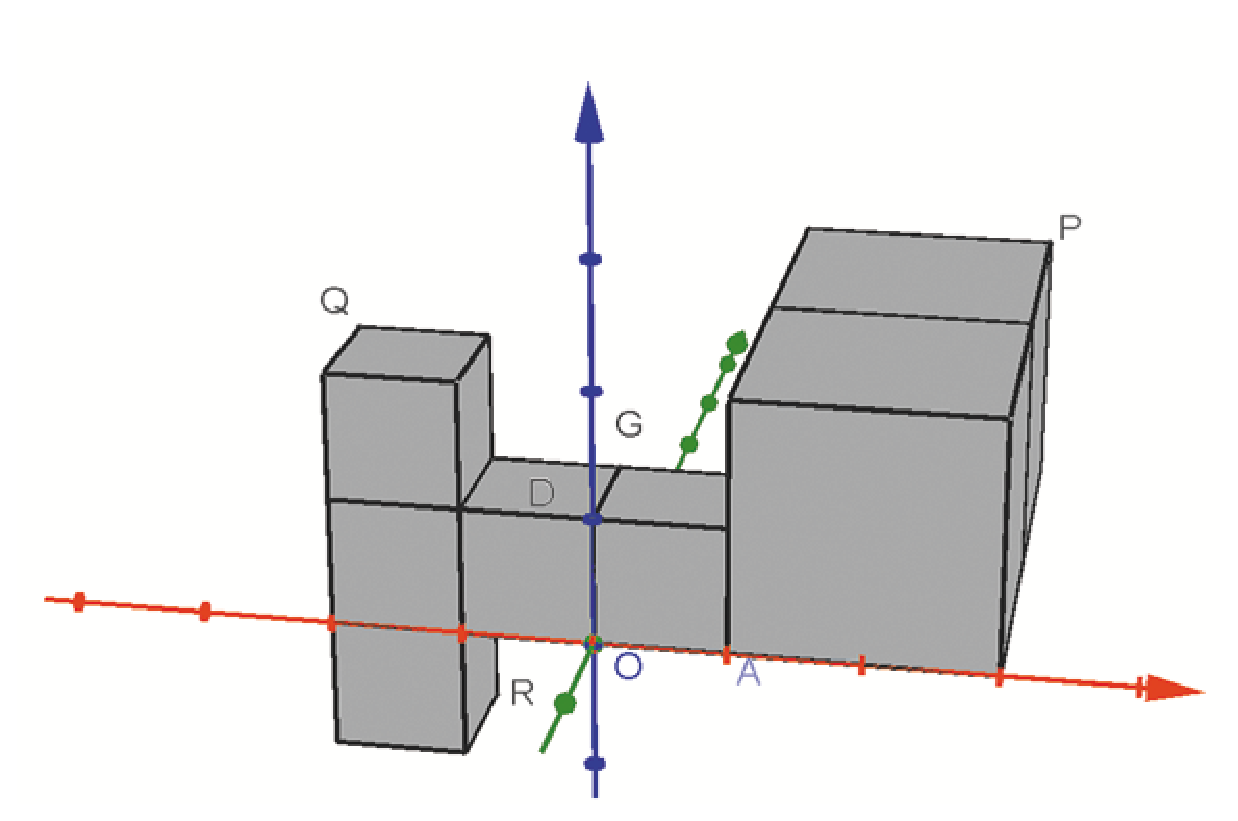
\includegraphics[scale=0.3]{RepE-flash4.eps}
\end{minipage}



\begin{DefT}{coordonnées sur une sphère}
\begin{minipage}{0.5\linewidth}

Si on assimile la Terre à une sphère, on peut repérer un point à sa surface par deux coordonnées correspondant à des mesures d'angles : La \textbf{latitude} et la \textbf{longitude}.
\begin{itemize}
\item Les \textbf{parallèles} sont des cercles dont les points ont la même latitude. La référence est l'équateur. Tous les points situés sur l'équateur ont pour latitude 0\deg .
\item Les \textbf{méridiens} sont des demi-cercles d'extrémités les pôles dont les points ont la même longitude. La référence est le méridien de Greenwich (Angleterre). Tous les points situés sur le méridien de Greenwich ont pour longitude 0\deg .
\end{itemize}
\end{minipage}
\begin{minipage}{0.5\linewidth}
\begin{center}
 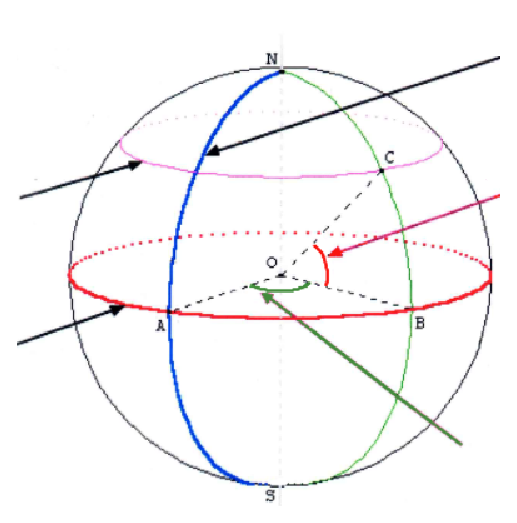
\includegraphics[scale=0.5]{lat_long_sphere.eps} 
\end{center}
\end{minipage}

\end{DefT}
 

\paragraphe{Perspective cavalière}




La perspective cavalière permet de représenter sur une surface en deux dimensions, un objet en trois dimensions. Quelques règles essentielles sont :
\begin{itemize}
\item Les traits pleins représentent les arêtes visibles.
\item Les traits en pointillés représentent des arêtes qui sont pas censées être vues. 
\item Les milieux sont conservés, le parallélisme est conservé.
\item Le plan de vue de face (plan frontal) conserve ses mêmes dimensions.
\end{itemize}




\paragraphe{Les volumes}

\begin{description}
\item[Volume du cube :]   \vplus
\item[Volume du cylindre :]  \vplus
\item[Volume du cône :]   \vplus

\item[Volume du pyramide :]   \vplus
\item[Volume du parallélépipède :]   \vplus
\item[Volume d'une sphère :]   \vplus
\end{description} 


\paragraphe{Théorèmes connexes}





\begin{ThT}{Théorème de Pythagore}
Dans un triangle rectangle, le carré de l'hypoténuse est égal à la somme des carrés des deux autres cotés.
\end{ThT}

On peut l'utiliser pour calculer une longueur dans l'espace.

 \vspace{1cm} 
 
\textbf{Application.}


\parbox{0.48\linewidth}{Pour présenter ses macarons, une boutique souhaite utiliser des présentoirs dont la forme est une pyramide régulière à base carrée de côté 30 cm et dont les
arêtes latérales mesurent 55~cm.

On a schématisé le présentoir par la figure ci-contre.

Calculer AO puis SO.
}\hfill \parbox{0.48\linewidth}{
\psset{unit=1cm}
\begin{pspicture}(5,4.5)
\pspolygon(0.5,0.5)(3.2,0.5)(4.5,2)(2.5,4)%ABCS
\psline(3.2,0.5)(2.5,4)
\psline[linestyle=dotted](0.5,0.5)(4.5,2)(1.8,2)(3.2,0.5)%ACDB
\psline[linestyle=dotted](0.5,0.5)(1.8,2)(2.5,4)
\psline[linestyle=dashed](2.5,4)(2.5,1.3)
\psline[linewidth=0.3pt](0.5,0.5)(1,0.5)(1.2,0.8)(0.7,0.8)
\psline[linewidth=0.3pt](3.2,0.5)(2.7,0.5)(2.9,0.8)(3.4,0.8)
\psline[linewidth=0.3pt](4.5,2)(4,2)(3.75,1.7)(4.25,1.7)
\psline[linewidth=0.3pt](1.8,2)(2.3,2)(2.1,1.7)(1.6,1.7)
\uput[dl](0.5,0.5){A} \uput[dr](3.2,0.5){B} \uput[ur](4.5,2){C} \uput[ul](1.8,2){D} \uput[d](2.5,1.3){O}\uput[u](2.5,4){S} 
\end{pspicture}
}

 
\begin{ThT}{Théorème de Thalès}

Dans un triangle ABC, tel que 
\begin{description}
\item[•] M appartient à (AB) et N appartient à (AC) 
\item[•](MN) est parallèle à (BC)  
\end{description}
alors : $ \frac{AM}{AB} =  \frac{AN}{AC} =  \frac{MN}{BC}$ 
\end{ThT}



On peut l'utiliser pour calculer une longueur dans l'espace.

 \vspace{1cm}
 
\textbf{Application.}

\parbox{0.65\linewidth}{La dernière bouteille de parfum a la forme
d'une pyramide SABC à base triangulaire de hauteur [AS] telle que :

$\bullet~~$ABC est un triangle rectangle et isocèle en A ;

$\bullet~~$AB = 7,5~cm et AS = 15~cm.

\medskip

Pour fabriquer son bouchon SS$'$MN, les concepteurs ont coupé cette pyramide par un plan P parallèle à sa base et passant par le point S$'$ tel que SS$'$ = 6~cm.

Calculer la longueur S$'$N.

} \hfill
\parbox{0.32\linewidth}{\psset{unit=0.75cm}
\begin{pspicture}(5.5,12)
%\psgrid
\pspolygon(0.4,1.4)(0.4,10.9)(3.2,0.5)%ASB
\psline(0.4,10.9)(5.2,1.4)(3.2,0.5)%SCB
\psline[linestyle=dashed](0.4,1.4)(5.2,1.4)%AC
\psline(0.4,7.1)(1.5,6.7)(2.3,7.1)%S'MN
\psline[linestyle=dashed](0.4,7.1)(2.3,7.1)%S'N
\psframe(0.4,1.4)(0.9,1.9)
\psline(0.9,1.4)(1.4,1.2)(1,1.2)
\uput[u](0.4,10.9){S}\uput[l](0.4,7.1){S$'$}
\uput[dr](1.5,6.7){M}\uput[r](2.3,7.1){N}
\uput[l](0.4,1.4){A}\uput[d](3.2,0.5){B}\uput[r](5.2,1.4){C}
\rput(2.6,1.4){$\circ$}\rput(2,0.9){$\circ$}
\end{pspicture}}







\end{document}